\chapter{Introduction}\label{ch:introduction}
The documentation for this project is split into four main parts.
The first chapter gives an introduction to some important features, technologies \& tools, keywords and notations that are crucial to this project.
It also covers the goals \& requirements that this project was initially set to meet.\\
\newline
The second chapter gives an overview and more thorough explanation on OpenRefine, the low code development platform for which the extensions have been built. TBD\\
\newline

The third (or main) chapter is split into two chapters for each of the extensions. These chapters explain about the actual technical implementation aspects of the extensions.
It mostly explains about the important methods/approaches that were used to achieve the goal of these extensions and the reason why those methods were decided to be used.
It also explains about the main technical notations about the project, what they mean and how they were used in the benefit of this project work.\\
\newline
The fourth and final chapter presents the results that were achieved from this project work and the outlook of it.
It also wraps up with a conclusion about the project and my personal reflection on this whole project work.
\newpage
\section{Requirements}
The main objective for this project is implementing different spatial data representations in OpenRefine and also integrating OpenStreetMap data into
a new OpenRefine project (one of the extensions). With the help of the other extension, geospatial data can be easily exported to the \textit{GeoJSON} format.\\
\newline
The main tasks include:
\begin{itemize}
   \item Creating an extension for OpenRefine that uses the Overpass API to fetch OpenStreetMap data and then integrate it into a new OpenRefine project.
    \subitem The OpenStreetMap data has to be converted to \texti{Simple Feature} Geometry (explained later in the paper).
    \subitem The XML data (received from Overpass) has to be converted to tabular data in order to comply with the OpenRefine schema.
   \item Creating an extension for OpenRefine that exports geospatial data into the \textit{GeoJSON} format.
    \subitem  The data can belong to any type of geometry and has to be of valid \textit{GeoJSON} format after the conversion.
\end{itemize}
The extensions stick to the official \href{https://docs.openrefine.org/technical-reference/writing-extensions}{OpenRefine development rules and guidelines for writing extensions}. They are licensed
under the \href{https://opensource.org/licenses/MIT}{MIT License}.
\newpage
\section{The Low Code Development Platform - OpenRefine}
OpenRefine (previously Google Refine) is a powerful tool for working with messy data: cleaning it; transforming it from one format into another; and extending it with web services and external data. \cite{AboutOpenRefine}\\
\newline
OpenRefine offers an extension architecture where users can extend the functionality of OpenRefine by creating various extensions.
The main requirements of this project are to build two extensions using OpenRefine's extension architecture in order to extend OpenRefine's functionality to
be able to import OpenStreetMap data into OpenRefine (\hyperref[{ch:the-osm-extractor-extension}]OSM Extractor)and also export geospatial
data into the GeoJSON format (\hyperref[ch:the-geojson-export-extension]{GeoJSON Export}).

\newpage
\section{Spatial Data}
The requirements of this project all work closely with spatial data and forms of its representation.\\
\newline
Spatial data, also known as geospatial data, is a term used to describe any data related to or containing information
about a specific location on the Earth\’s surface. \cite{AboutGeoSpatialData}\\
\newline
Geospatial data is data about objects that have a location on the surface of the Earth.
Locations can be static or dynamic. Static data are locations that don't move such as restaurants, roads or buildings.
Dynamic data are locations that move/change with time e.g. a moving vehicle, the spread of a disease etc.\\
\newline
Much of the geospatial data around the world is available as open data. This means that it can be freely accessed by the people
around the world who can use it to their own interest. Geospatial organizations have invested and supported the promotion of
geospatial data a lot recently, a lot of small agencies contribute daily to the collection of geospatial data around the world.
There are a lot of non-profit organizations that support the development of open geospatial data by offering different standards
for representing the data and tools for working with such data. Some of these organizations include: The \href{https://www.ogc.org/}{Open Geospatial Consortium (OGC)},
\href{https://www.esri.com/en-us/home}{ESRI}, the \href{https://www.osgeo.org/}{Open Source Geospatial Foundation (OSGeo)},
the \href{https://www.iso.org/home.html}{ISO organization} etc.\\
\newline
Geospatial data can be represented in many ways, as mentioned above, a lot of organizations have standardized the ways of representing
such data. For example, exact locations on the map (or points) can be represented simply by their X and Y coordinates, also known as longitude and latitude.
More complex geographic objects such as highways or train stations have multiple ways of representations, in this project however, such representations
are done using the \textit{Well-Known Text (WKT)} representation. Well-Known Text or WKT is a text representation for exchanging geometry data, originally developed by
the \href{https://www.ogc.org/}{Open Geospatial Consortium (OGC)} and described in their \href{https://www.ogc.org/standards/sfa#overview}{Simple Feature Access}.
More technical details about WKT and how this project utilizes it will be provided in the implementation chapters.\\
\newline
\newpage
\section{OpenStreetMap \& the Overpass API}
\subsection{OpenStreetMap}
OpenStreetMap is powered by open-source software such as editing software, various APIs etc.
One can extract very sophisticated information from the geographical data the OSM consists of.
Various users (end-users, developers, maintainers etc.) all around the world contribute daily to improving the geographical
data in OSM and to improving the ease of use of such data and information.
The OSM data can be used in multiple ways such as producing paper and electronic maps,
integrating such data into your own applications and route planning.\\
\newline

There are already a lot of famous users that utilize OSM such as:
\href{https://www.facebook.com/}{Facebook},
\href{https://www.craigslist.org/}{Craigslist},\href{https://www.seznam.cz/}{Seznam} etc.
OSM is \textit{community-driven} and the community of contributors mainly consists of enthusiast mappers,
GIS professionals, humanitarians and many more. It is also \textit{open-data}, which means that anyone can freely use
OSM for any purpose as long as OSM and its contributors are credited.
The OSM map data ca be used for web sites, mobile apps and various hardware devices.\\
\newline
OpenStreetMap is freely accessible by the people around the world on \href{https://www.openstreetmap.org/}{https://www.openstreetmap.org/}\\
\newline
\begin{figure}[H]
    \centering
    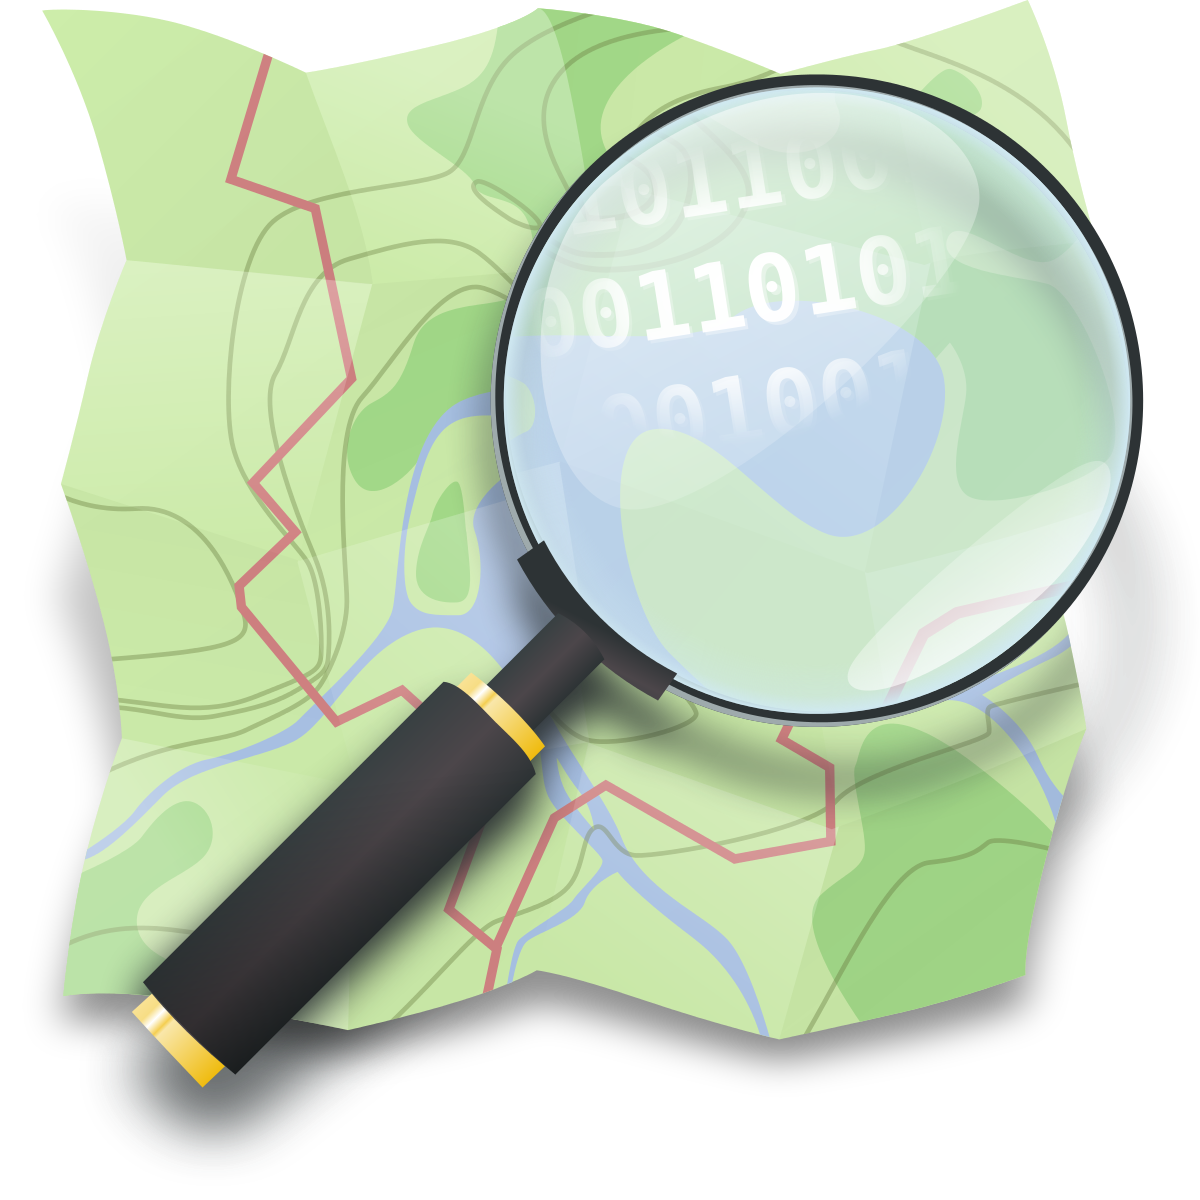
\includegraphics[width=5cm]{./Figures/Introduction/openstreetmap_logo.png}
    \caption{The OpenStreetMap logo}
\end{figure}
\newpage
\subsection{The Overpass API}
\href{https://wiki.openstreetmap.org/wiki/Overpass_API}{The Overpass API} (formerly known as OSM Server Side Scripting,
or OSM3S before 2011) is a read-only API that serves up custom selected parts of the OSM map data.
It acts as a database over the web: the client sends a query to the API and gets back the data set that corresponds to
the query. \cite{WhatIsOverpass}\\ The Overpass API is mainly optimized for querying OpenStreetMap elements instantly
which are selected by search criteria e.g. tags, locations etc.\\
\newline
In this project, the Overpass API is used to fetch OpenStreetMap data (elements) by using the
\href{https://wiki.openstreetmap.org/wiki/Overpass_API/Overpass_QL}{Overpass QL} querying language in order to
retrieve the desired data from OpenStreetMap.\\
\newline
\begin{figure}[H]
    \centering
    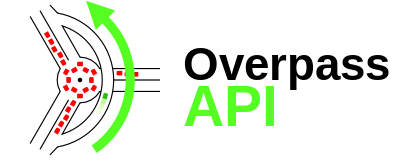
\includegraphics[width=5cm]{./Figures/Introduction/overpass_api.png}
    \caption{The Overpass API logo}
\end{figure}
\newpage
\section{GeoJSON}
\href{https://geojson.org/}{GeoJSON} is a format based on the JSON format which is designed for representing \href{https://www.ogc.org/standards/sfa#overview}{simple geographical features}
along with their properties.\\
\newline
GeoJSON supports the following feature types:
\begin{itemize}
    \item Point (including addresses and locations)
    \item Line string (including streets, highways, and boundaries)
    \item Polygon (including countries, provinces, and tracts of land)
    \item Multipart collections of point, line string, or polygon features
\end{itemize}
GeoJSON features are not only used to represent entities of the physical world. For example, mobile routing and navigation apps
might describe their service coverage using GeoJSON. \cite{ArcGISGeoJSON}\\
\newline
One of the extensions on this project does the job of converting OpenRefine data (geospatially represented) into the \href{https://geojson.org/}{GeoJSON (.geojson)} format.